% Appendix A

\chapter{Levels of Automation by Sheridan and Verplank} % Main appendix title

\label{AppendixA} % For referencing this appendix elsewhere, use \ref{AppendixA}


\begin{figure}
    \centering
    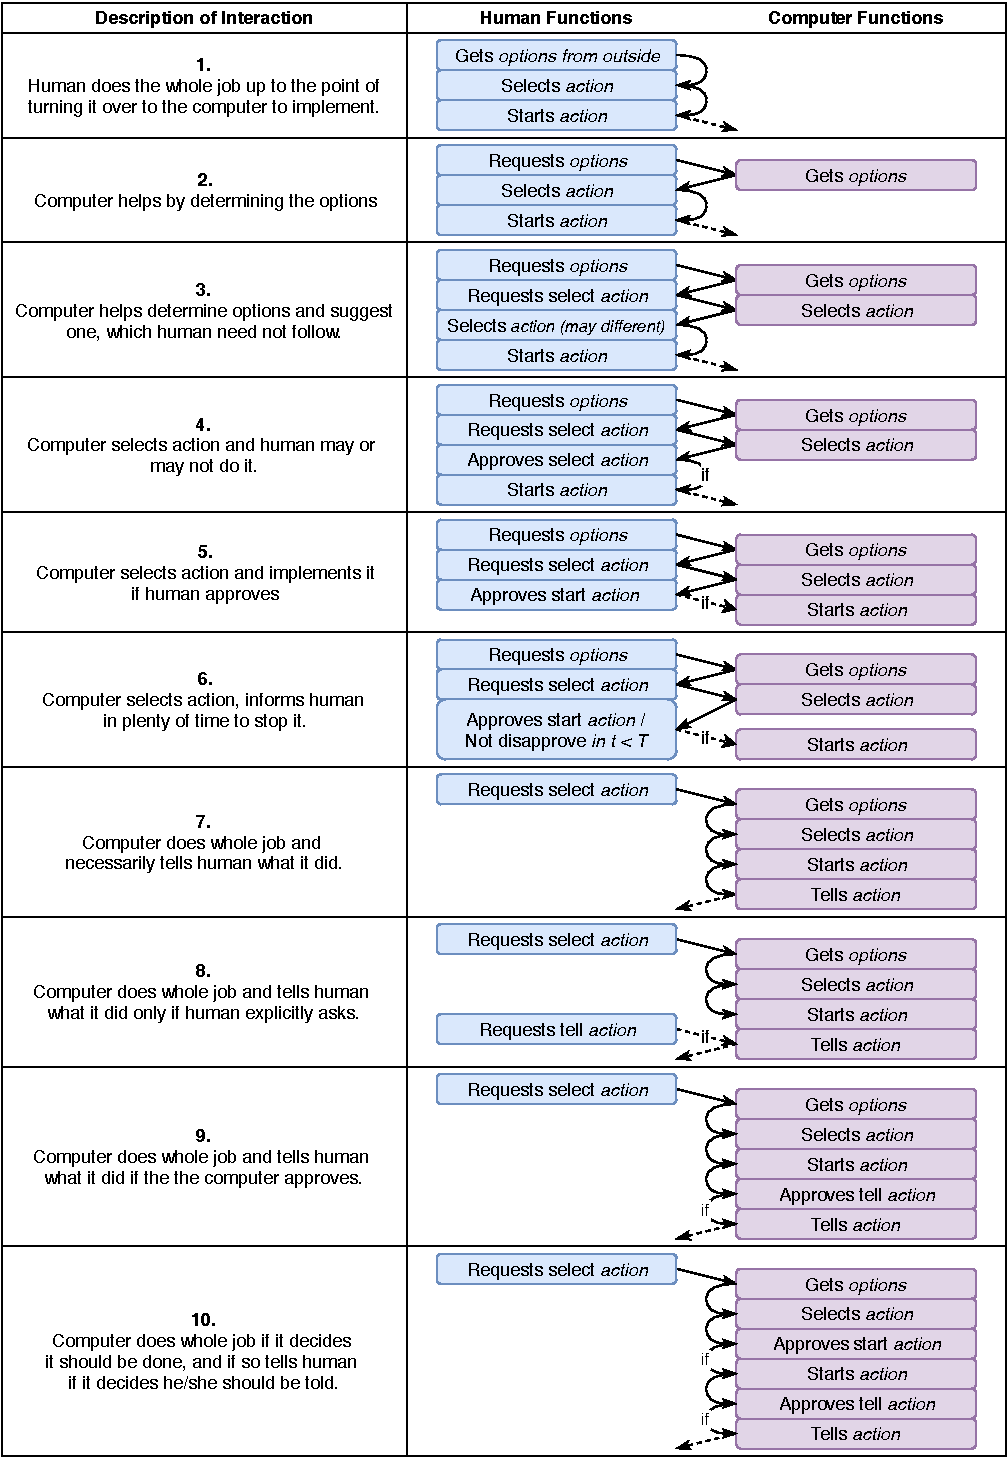
\includegraphics[width=\textwidth]{Figures/draw.io/levels_of_automation_in_man-computer_decision_making_for_a_single_elemental_decisive_step}
    \decoRule
    \caption[Levels of automation in man-computer decision making for a single elemental decisive step]{Levels of automation in man-computer decision making for a single elemental decisive step. \textit{Source: table 8.2 from \cite{Sheridan1978} (edited), created with \href{https://www.draw.io/}{draw.io}}}
    \label{fig:levels_of_automation_in_man-computer_decision_making_for_a_single_elemental_decisive_step}
\end{figure}

%\begin{table}
%    \caption[Levels of Automation in Man-Computer Decision-Making by Sheridan and Verplank]{Levels of Automation in Man-Computer Decision-Making by Sheridan and Verplank. \textit{Source: table 8.2 from \cite{Sheridan1978}, edited.}}
%    \label{tab:Levels_of_Automation_by_Sheridan_and_Verplank}
%    \centering
%    \begin{tabular}{r p{0.8\textwidth} l }
%    \toprule
%    \tabhead{Level} & \tabhead{Definition} \\
%    \midrule
%    1   & The Human remote-controls the UAV and makes all decisions and actions without any assistance from the computer.                      \\
%    2   & The Computer assists the human with decision making by providing a full set of all alternative decisions/actions.                 \\
%    3   & The Computer assists the human with decision making by selecting a subset of alternative decisions/actions.          \\
%    4   & The Computer makes decisions by choosing a single alternative decision/action.                       \\
%    5   & The Computer executes its chosen alternative decision/action, if the human approves.                                     \\
%    6   & The Computer executes its chosen alternative decision/action, if the human does not disapprove in a specified time span.             \\
%    7   & The Computer certainly executes its chosen alternative decision/action and informs the human.                            \\
%    8   & The Computer certainly executes its chosen alternative decision/action and informs the human if he/she requires.                             \\
%    9   & The Computer certainly executes its chosen alternative decision/action and decides whether to inform the human.                             \\
%    10  & The Computer makes all decisions/actions autonomously and ignores the human.                         \\
%    \bottomrule\\
%    \end{tabular}
%\end{table}